\documentclass[10pt,onecolumn,journal,draftclsnofoot]{IEEEtran}
\usepackage[margin=0.75in]{geometry}
\usepackage{listings}
\usepackage{color}
\usepackage{longtable}
\usepackage{graphicx}
\usepackage{float}
\usepackage{tabu}
\usepackage{enumitem}
\usepackage{courier}
\usepackage{hyperref}
\usepackage{parskip}
\definecolor{dkgreen}{rgb}{0,0.6,0}
\definecolor{gray}{rgb}{0.5,0.5,0.5}
\definecolor{mauve}{rgb}{0.58,0,0.82}

\lstset{frame=none,
language=C,
columns=flexible,
numberstyle=\tiny\color{gray},
keywordstyle=\color{blue},
commentstyle=\color{dkgreen},
stringstyle=\color{mauve},
breaklines=true,
breakatwhitespace=true,
tabsize=4,
showstringspaces=false,
basicstyle=\ttfamily
}

\setlength{\parindent}{0cm}

\begin{document}
\begin{titlepage}
  \pagenumbering{gobble}
  \title{POWER8 Continuous Integration\\ Spring Midterm Progress Report}
  \author{Leon Leighton, Thomas Olson, Derek Wong\\Project 35}
  \date{May 15, 2017}
  \maketitle
  \vspace{4cm}
  \begin{abstract}
  \noindent This document contains an overview of the progress of the POWER8 Continuous Integration project.
    It includes the goals and purpose of the project, the current status, items remaining to be done, 
    and a discussion of problems we have encountered. 
 \end{abstract}
\end{titlepage}

\pagenumbering{arabic}
\tableofcontents
\clearpage

\section{Project Goals}
The primary goal of this project is to create a continuous integration (CI) system for IBM's POWER8 architecture.
This CI system will be available to open source software projects, giving them the ability to build and test their software on POWER8 without the need for them to acquire new hardware.
We will be utilizing the OSU Open Source Lab's POWER8 OpenStack cluster to deploy our project and run the builds and tests.
We also aim to make the system easy to use while still giving users the ability to customize their build environment.
Our focus will be on interacting with GitHub to trigger new builds as developers commit new changes to their code.
Users will be able to access the status of their builds to gain information about build or test failures.
They will also be able to download the binaries built by the system.
Our project will also be open source and hosted on GitHub which will allow others to replicate our project on their own systems.

\section{Current Progress}
Our project is currently feature complete with a few bugs and requested changes remaining to be resolved.
We currently have two virtual machines running on the OSL's POWER8 OpenStack cluster.
One serves as the Jenkins and web host, and the other serves as a Docker host. 
In addition, at any given time, multiple build VMs may be running to service Jenkins jobs that have requested to be built in a separate virtual machine rather than in a Docker container.\\
\begin{figure}[H] 
  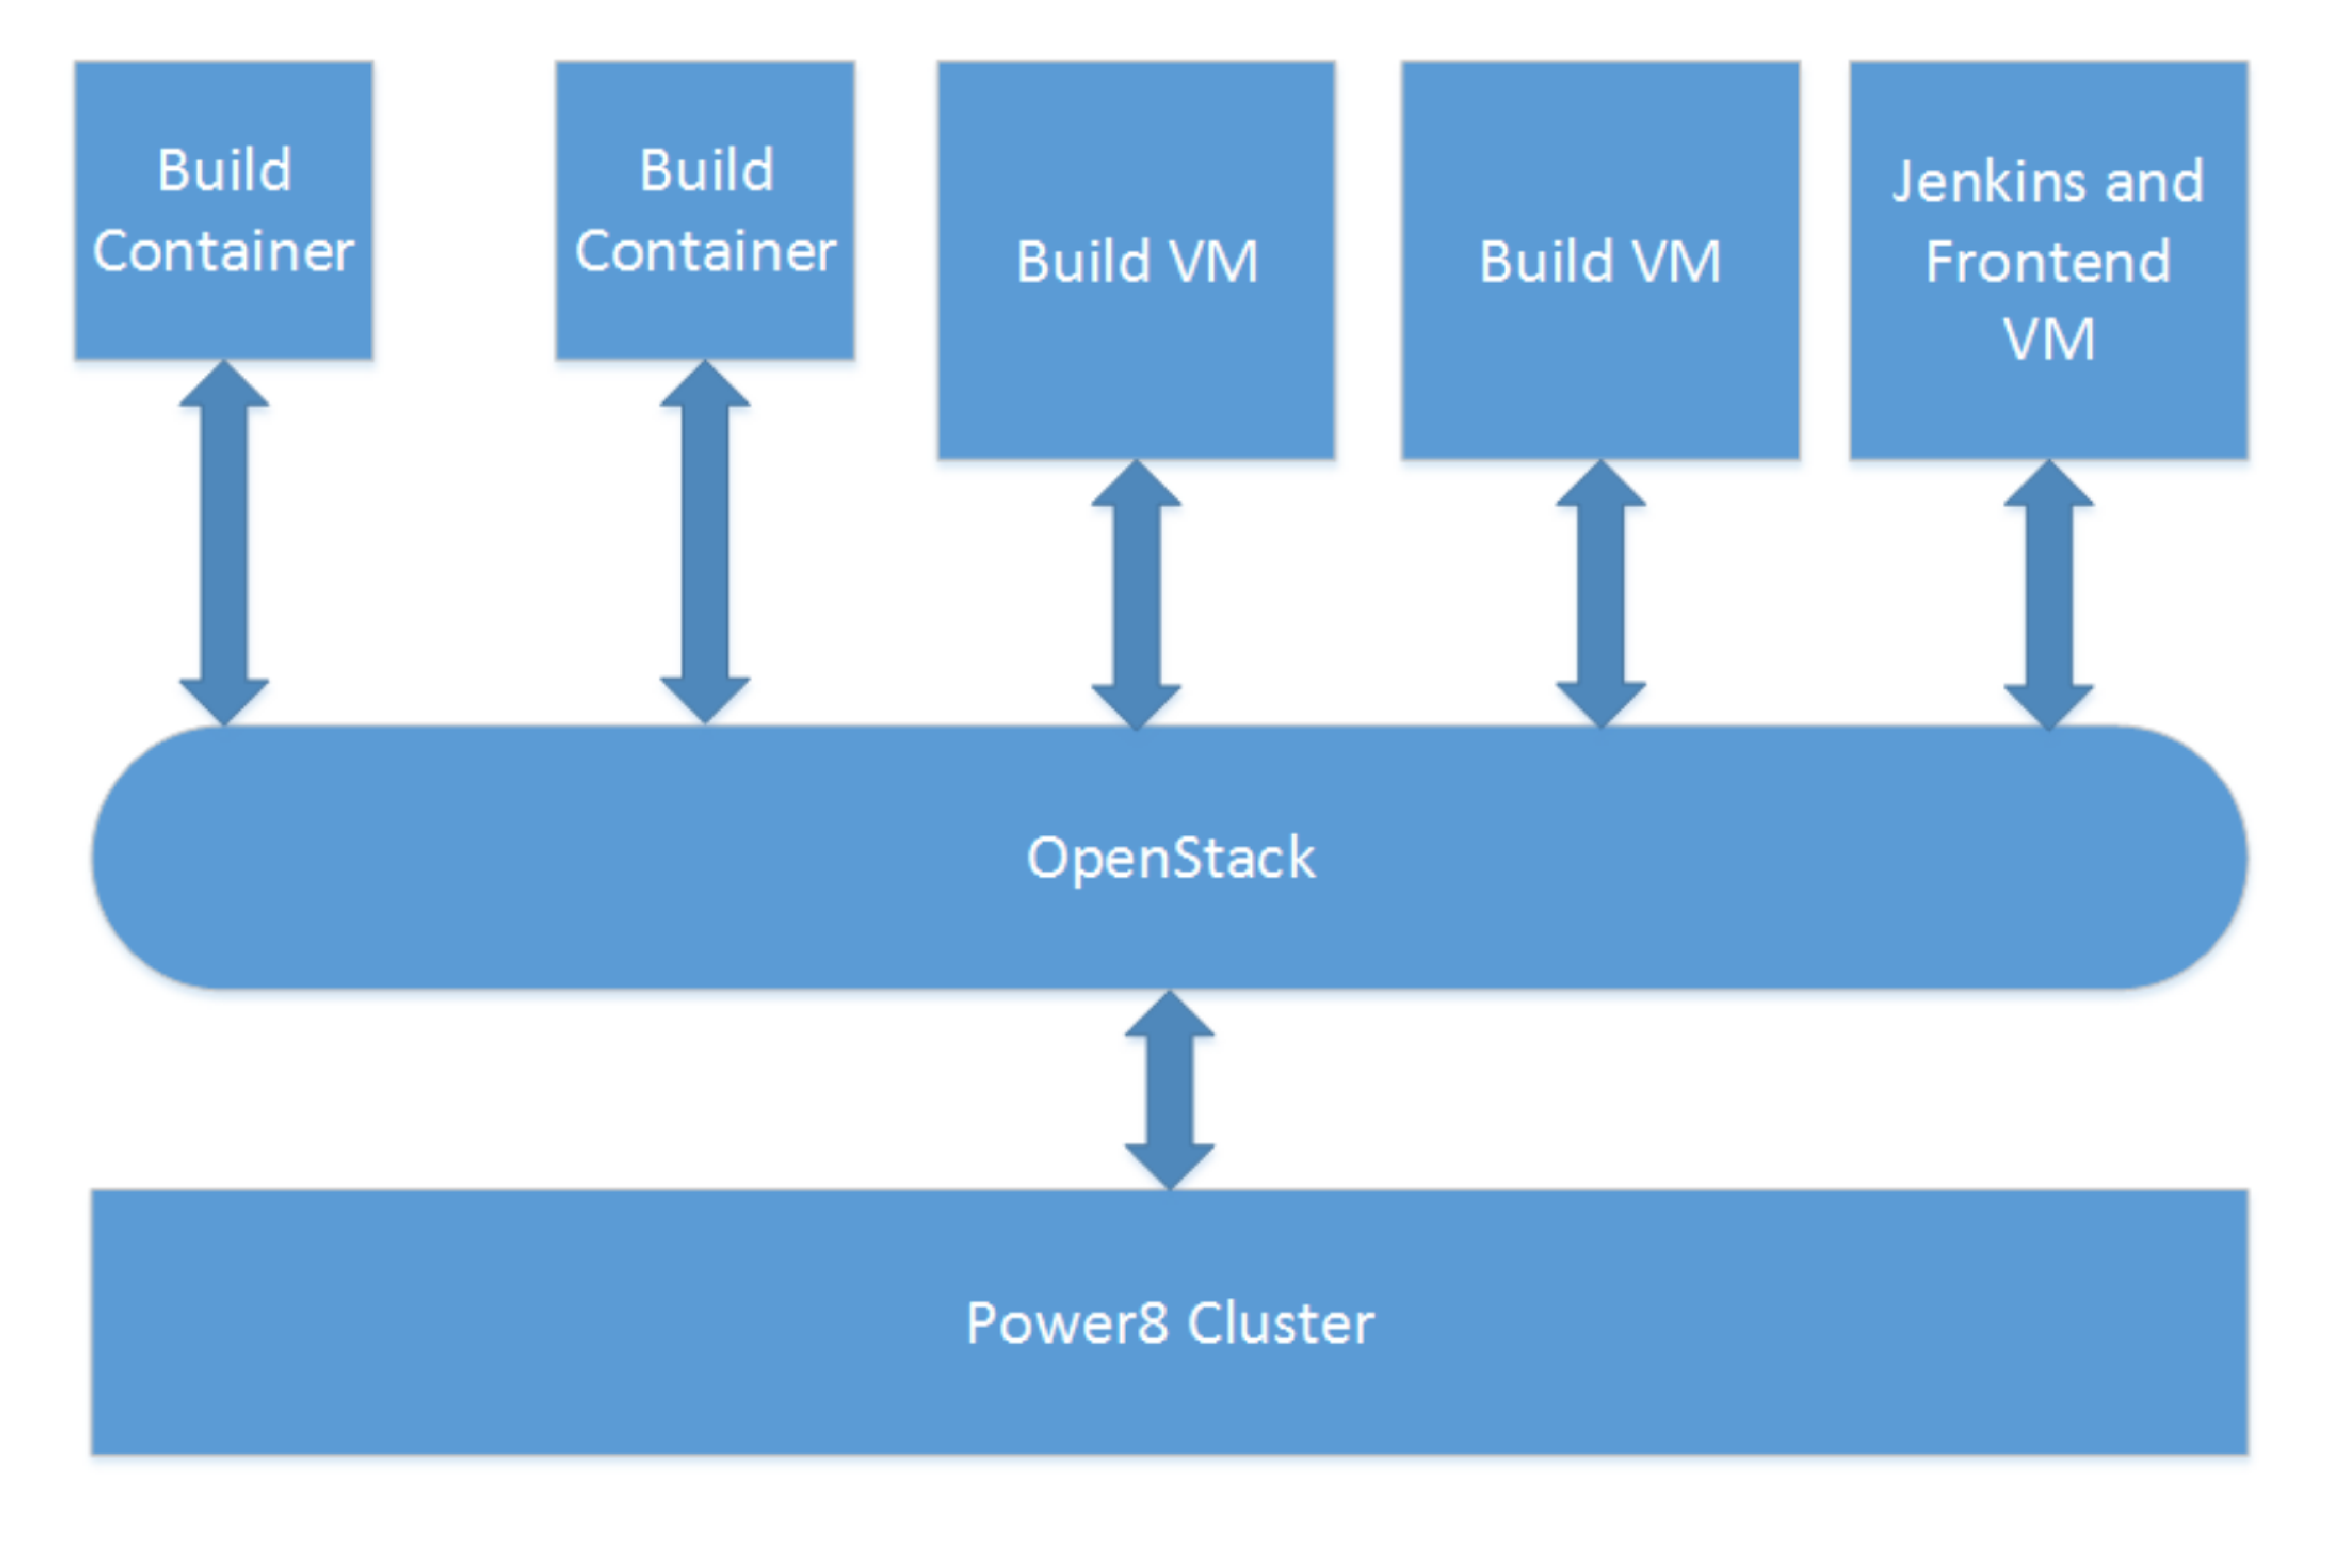
\includegraphics[width=\textwidth]{images/infrastructure_diagram.eps}
  \caption{POWER8 CI Infrastructure Diagram}
\end{figure}

We use Ansible to install and configure Jenkins, Jenkins plugins, and our web site.
Using Ansible gives us a reproducible deployment of our system and documentation of what we have installed and configured.
Keeping our Ansible playbook on GitHub makes it available to others who may want to deploy their own CI system based on our work.

\begin{lstlisting} [caption={Ansible playbook to install and configure Jenkins, Jenkins plugins, and the power-ci web page}]
- name: Install and configure Jenkins
  hosts: jenkins
  roles:
    - geerlingguy.jenkins
    - jenkins
    - web
  remote_user: ubuntu
  become: yes
  vars_files:
    - group_vars/jenkins
\end{lstlisting} 
Jenkins is the primary means of automating builds, and the Jenkins interface is where users create and configure their builds.
Depending on options selected by the user, Jenkins will direct the Docker host to start a container or direct OpenStack to start
a new virtual machine. 
Currently, Docker is the default if no option is selected by the user.

\begin{figure}[H] 
  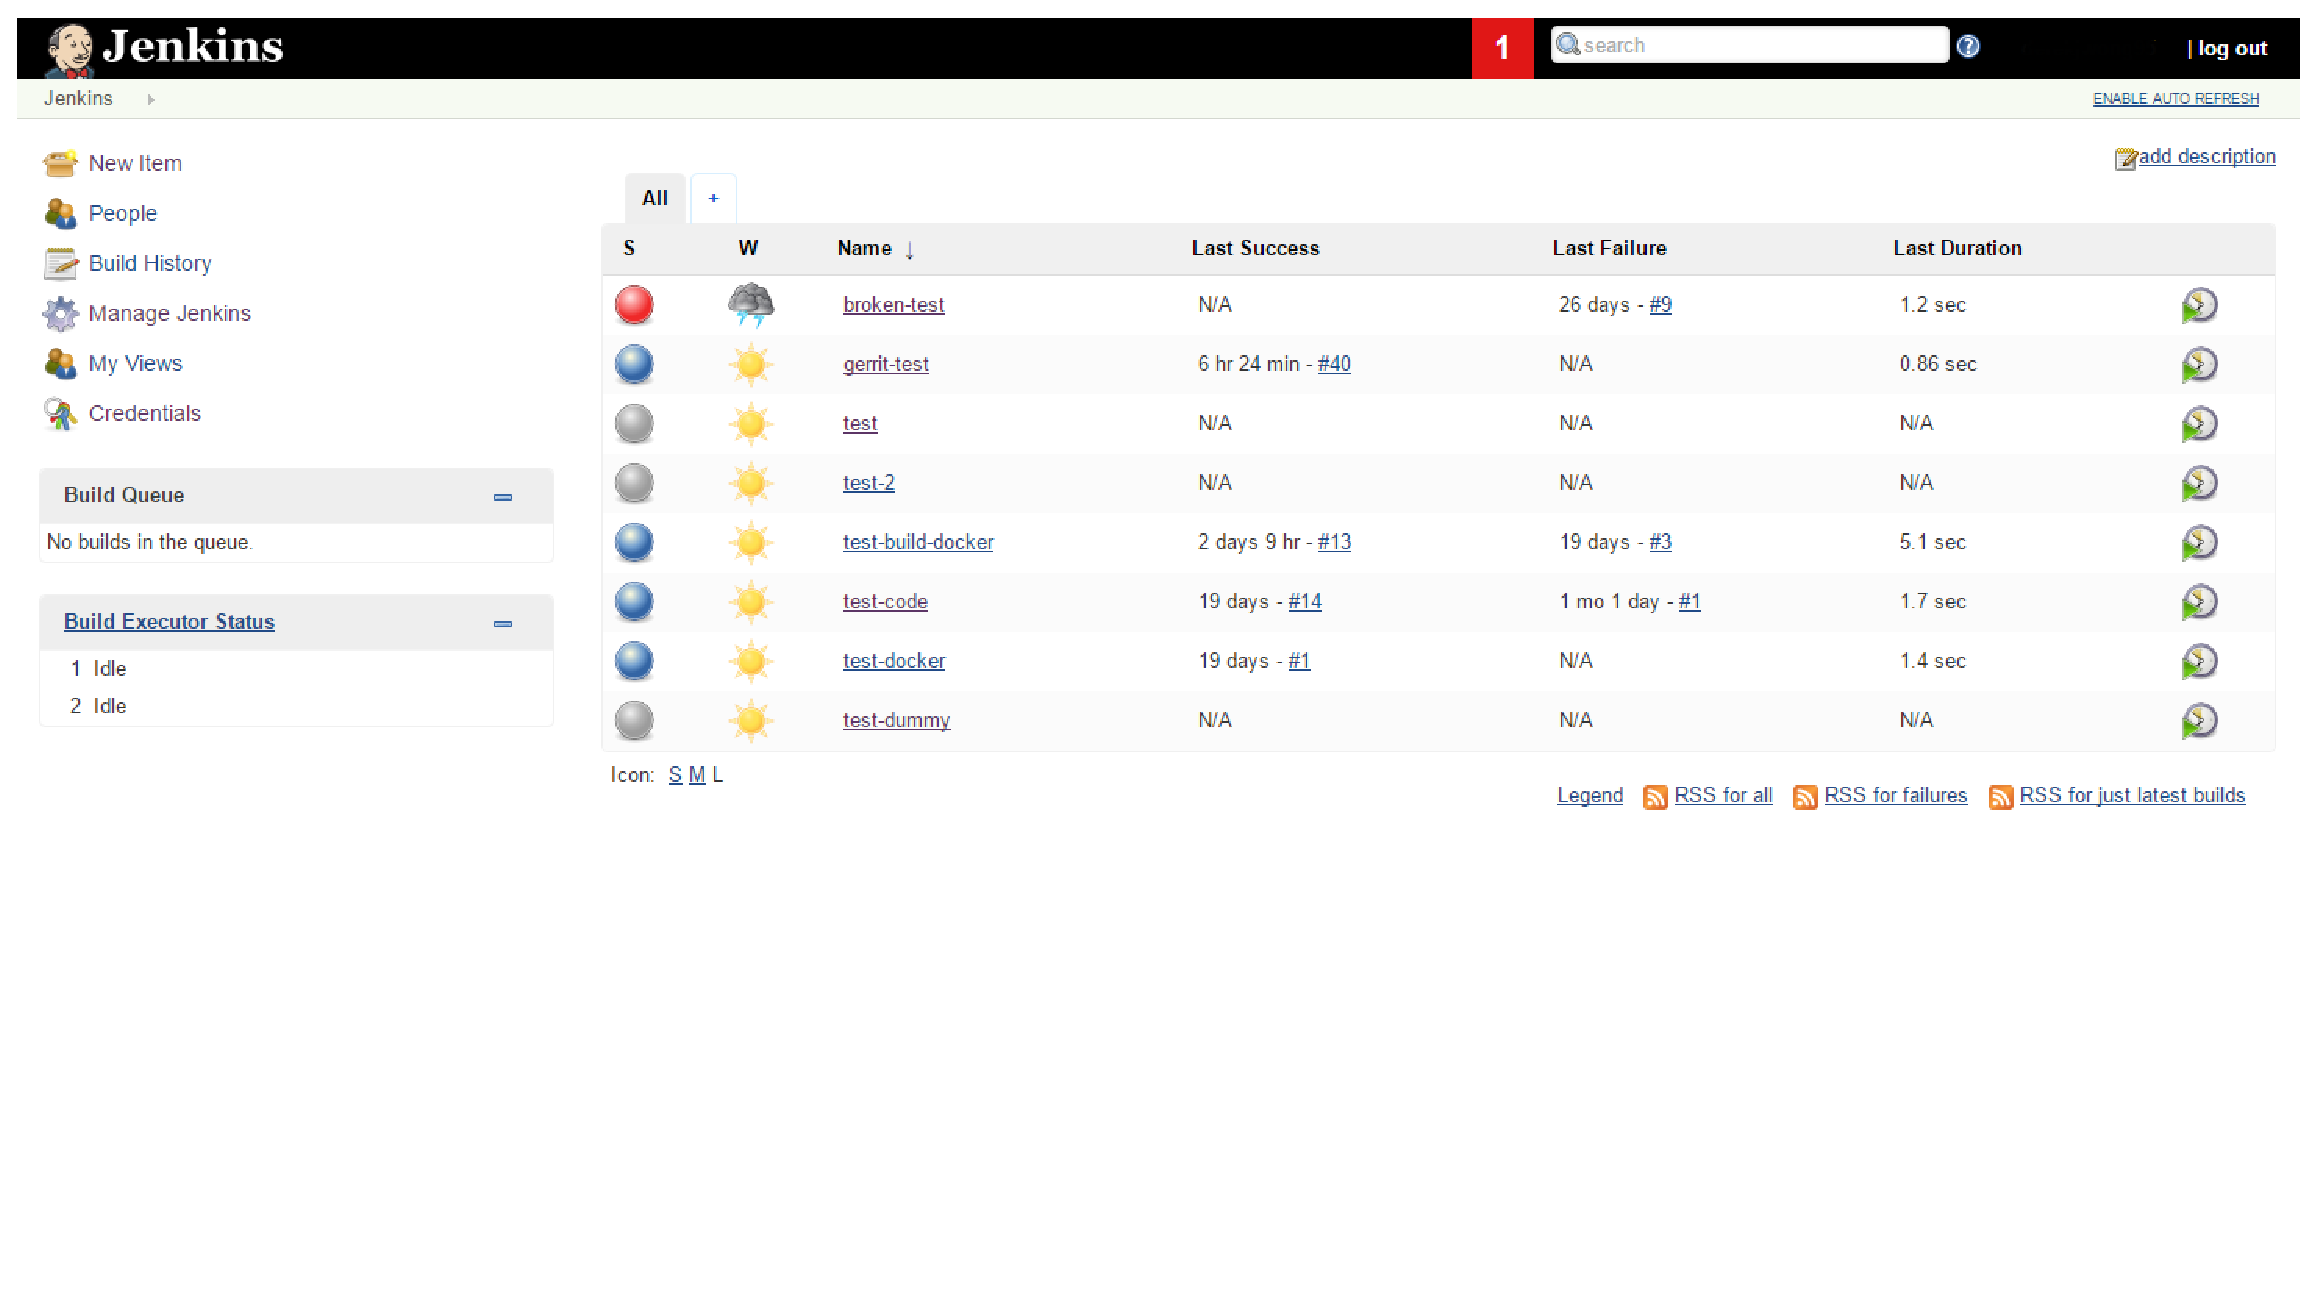
\includegraphics[width=\textwidth]{images/jenkins.eps}
  \caption{Jenkins Interface}
\end{figure}
\clearpage
We make extensive use of existing Jenkins plugins.
The GitHub OAuth Plugin is used for authentication allowing our users to login to our service with their GitHub account.
For authorization, we are using the Matrix Authorization Strategy Plugin to give users the permissions that they need to run their builds and tests.
The Build Monitor, Embeddable Build Status, and the Email Notification plugins are used to communicate the status of Jenkins jobs to the user.
The Embeddable Build Status Plugin is used to create a GitHub Badge and will allow developers to see their build status on their project's GitHub page.
The Email Notification Plugin can be used to send an email to the developers whenever a build is broken.
The Build Monitor Plugin can be used to create a view that can give a user an overview of all their projects and their statuses.

To provide isolation between Jenkins jobs we use the Docker, CloudBees Docker Build and Publish, OpenStack, and Job Restriction plugins. 
The Docker and CloudBees Docker Build and Publish plugins enable the use of either a pre-built container image, or a user supplied Dockerfile.
The OpenStack Plugin allows a user to run their build in a completely separate VM which provides the maximum amount of isolation between project builds. 
The Job Restriction Plugin allows us to enforce building in either a Docker container or a VM, and allows us to prevent building jobs on the Jenkins instance itself. 

Jenkins, the various Jenkins plugins, and the integration with GitHub, Docker, and OpenStack come together to create a Continuous Integration system.
The following workflow diagram shows how these pieces fit together to support building and testing on POWER8.

\begin{figure}[H] 
  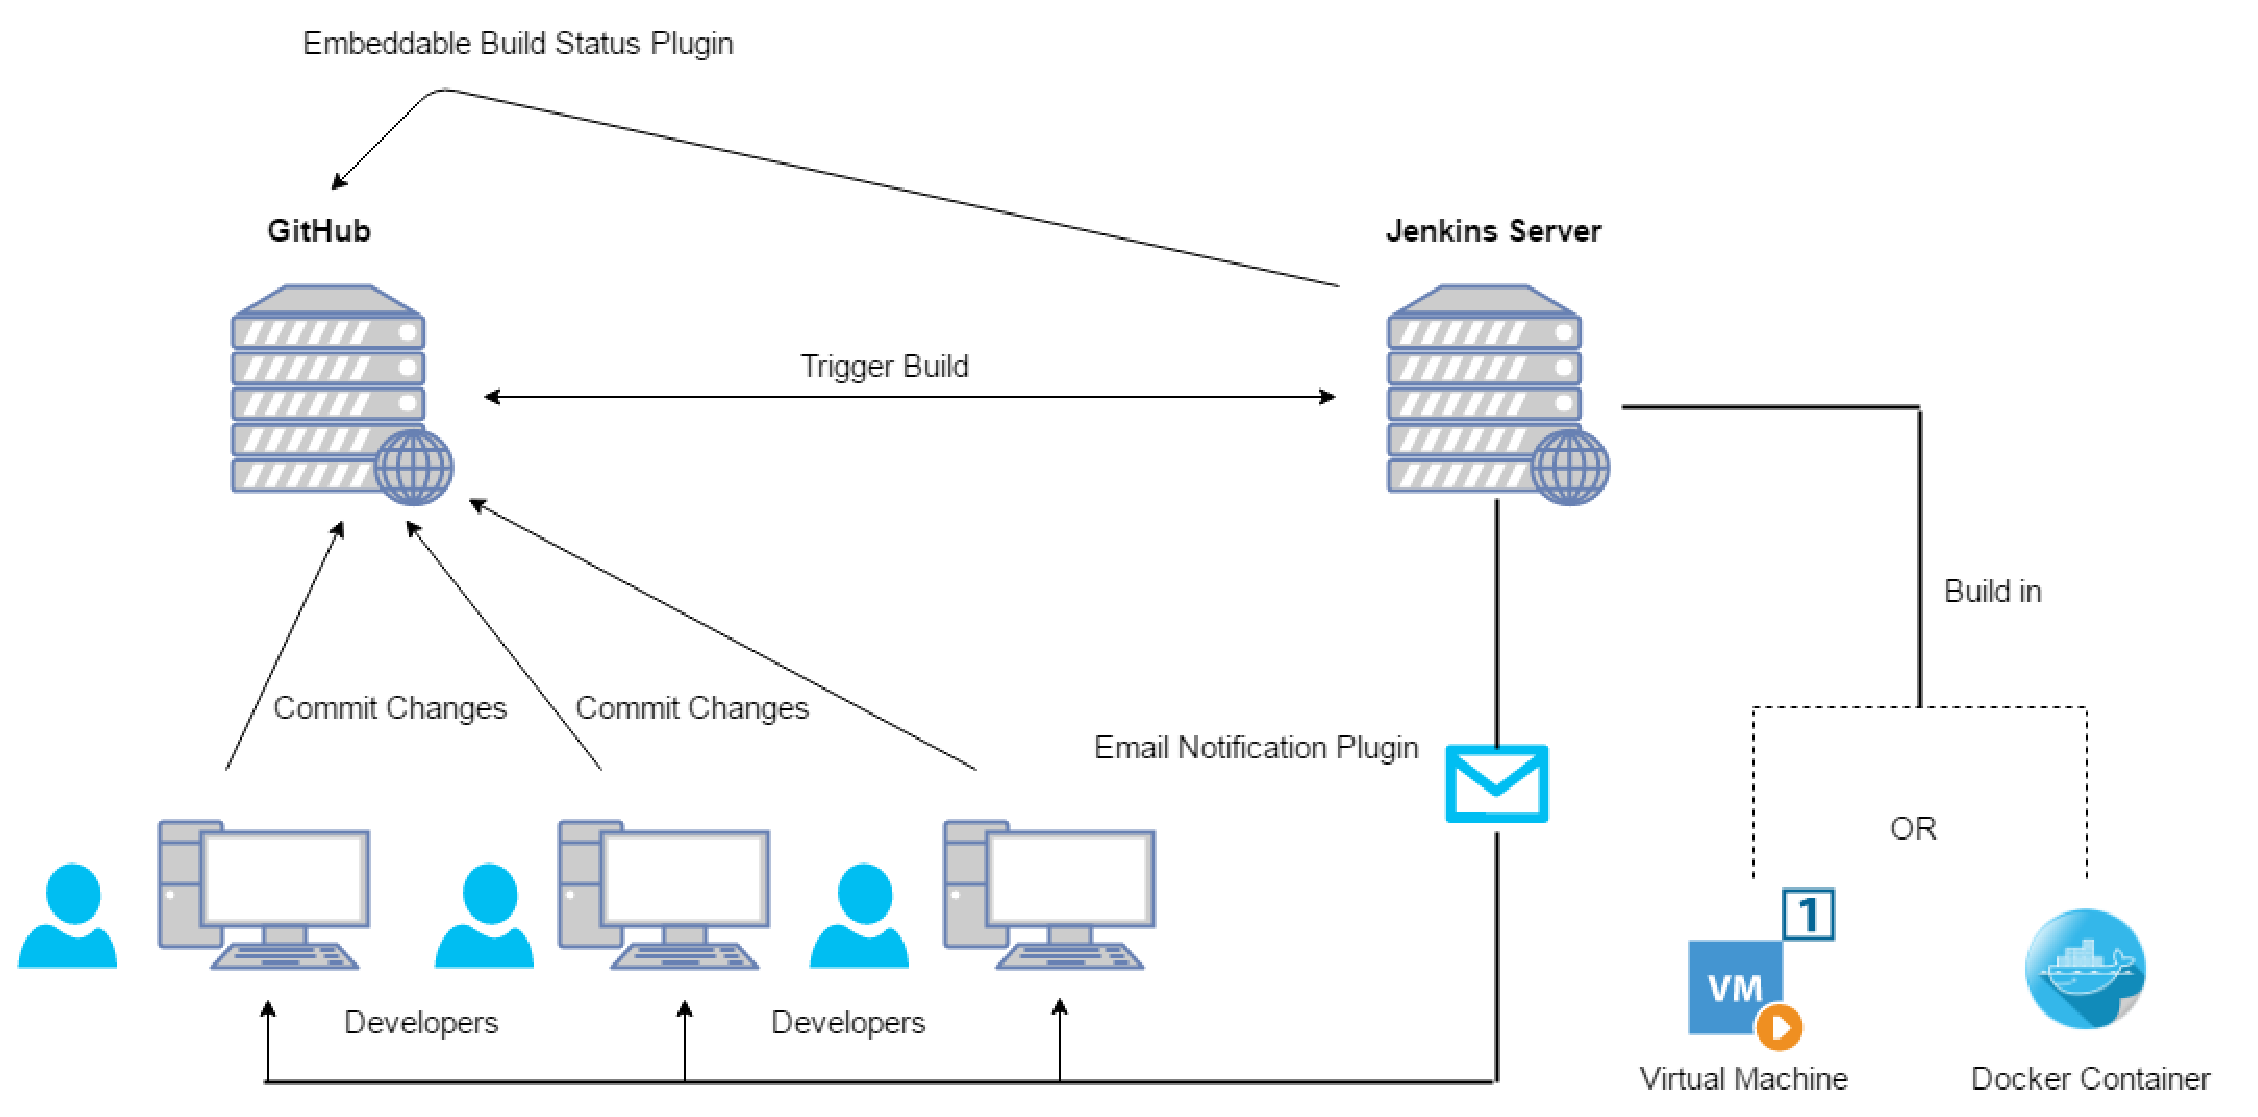
\includegraphics[width=\textwidth]{images/workflow.eps}
  \caption{POWER8 CI Workflow Diagram}
\end{figure}

\clearpage
\section{Remaining Items}
We have a few items remaining to be done before the end of the capstone project.
We expect to have all of the following items done soon, but they are not complete at the time of writing this progress report.
The first item is to use the Apache web server as a reverse proxy to the Jenkins interface.
This change would allow us to use TLS to secure the login to Jenkins, as well as remove the need to use an alternate port number. 
That is, instead of using http://power-ci.osuosl.org:8080 to access Jenkins, one would use https://power-ci.osuosl.org/jenkins. 
Another item is to use our web site, https://power-ci.osuosl.org, to host basic documentation about the use of the system.
This would include information about how to request access and what abilities our service provides.
Also, relevant links to existing Jenkins documentation will be provided. 
A third item to be completed is the onboarding process itself. 
After discussions with IBM and the OSL, we will be making a change to the existing PowerLinux / OpenPOWER Request Form at http://osuosl.org/services/powerdev/request\_hosting/ to allow projects the ability to request access to the POWER8 CI system and get the GitHub username that should be added to the system. 
This request will go to the OSL and IBM for approval before access is granted.
The final item that we are in the process of, but remains to be completed, is to continue to build more complicated jobs to find and resolve any bugs.
For obvious reasons, we started with very simple Jenkins jobs to ensure the basic functioning of our CI system.
However, more complicated builds enable us refine needed components of our Docker container and virtual machine images, as well as any permission issues within Jenkins itself.


\section{Problems and Solutions}
This term we have run into two problems which slowed our progress.
The first is not taking full advantage of the resources available from IBM\@.
IBM has employees who have worked with Jenkins, Docker, and Ansible.
It would have been to our benefit to reach out earlier in the process to these resources to help resolve configuration problems that we encountered.
By not taking advantage of these available resources it has taken us longer to solve problems, and we may have missed better solutions to those problems.
The second problem we encountered was not having a wide variety of test builds.
As we open up our project to the public we want to be confident that they will not run into any problems in using our CI service.
Different builds that have different requirements and complexities can show us where our virtual machine and Docker container images are lacking needed resources or configurations. 
If we had prioritized having a variety of builds earlier we would have been solving some of the problems we have only encountered more recently at an earlier stage of development.

To attempt to solve these problems we have been working closer with IBM to get a variety of builds to test on our CI system.
We have been given builds that IBM has been running internally on their Jenkins infrastructure.
At first, these builds failed on our system, but we were able to identify and fix the problems.
IBM has also reached out to other projects to see if any are interested in beta testing our CI system.
These projects were identified as already using virtual machines available from the OSL to run their own CI system on POWER8.
We are currently waiting to hear back from those projects.
\end{document}
